\documentclass{standalone}

\usepackage[landscape]{geometry}
\usepackage{amsmath}
\usepackage{amssymb}
\usepackage{pgfplots}
\usepackage{xcolor}

\geometry{letterpaper, margin=2.5cm}

\begin{document}
    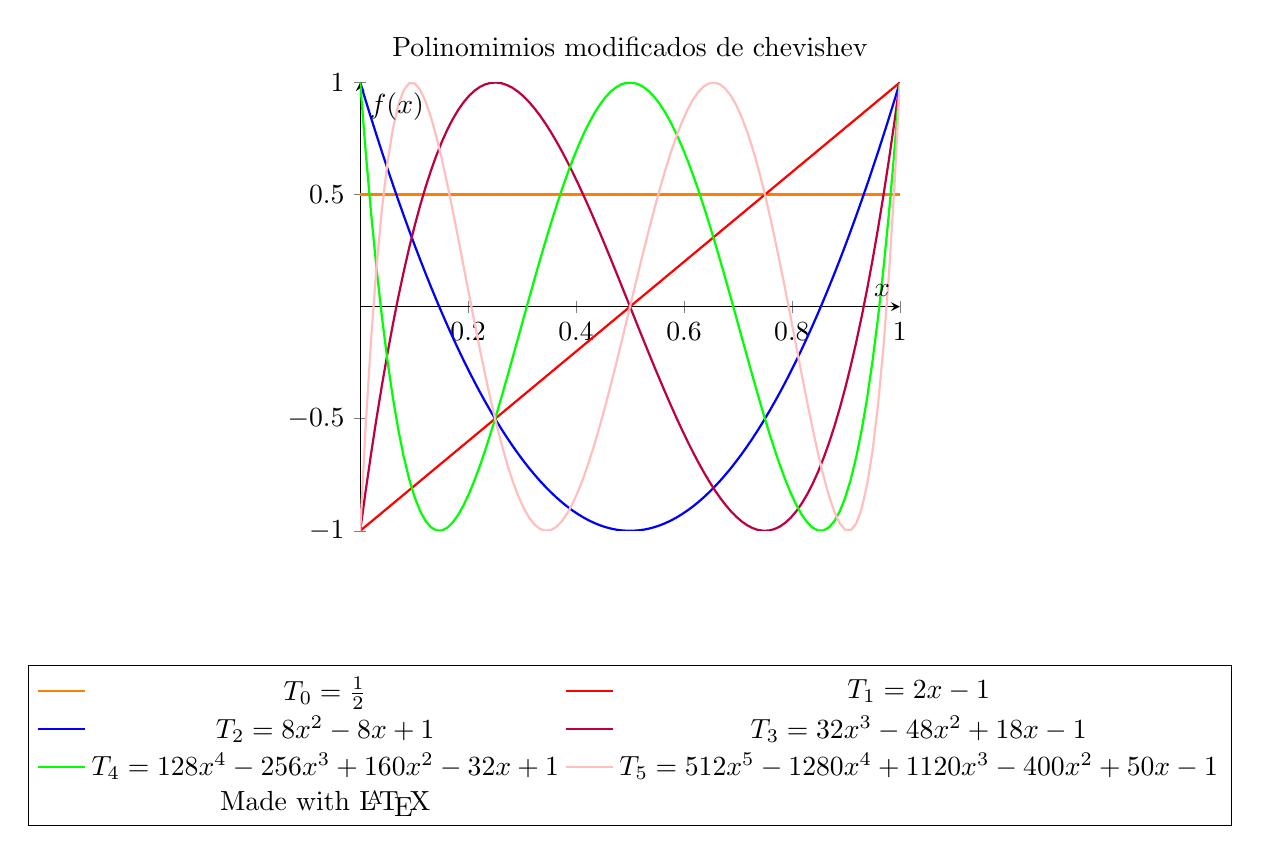
\begin{tikzpicture}
        \begin{axis}[
            title={Polinomimios modificados de chevishev},
            axis lines = middle,
            xlabel={$x$},
            ylabel={$f(x)$},
            xmin=0, xmax=1,
            ymin=-1, ymax=1,
            samples=100,
            domain=0:1,
            legend style={at={(0.5,-0.3)}, anchor=north, legend columns=2}
        ]
            \addplot[orange, thick] {0.5};
            \addlegendentry{$T_{0} = \frac{1}{2}$}
            \addplot[red, thick] {2*x-1};
            \addlegendentry{$T_{1} = 2x-1$}
            \addplot[thick, blue] {8*x^2-8*x+1};
            \addlegendentry{$T_{2} = 8x^{2}-8x+1$}
            \addplot[purple, thick] {32*x^3-48*x^2+18*x-1};
            \addlegendentry{$T_{3} = 32x^{3}-48x^{2}+18x-1 $}
            \addplot[green, thick] {128*x^4-256*x^3+160*x^2-32*x+1};
            \addlegendentry{$T_{4} = 128x^4-256x^3+160x^2-32x+1 $}
            \addplot[pink, thick] {512*x^5-1280*x^4+1120*x^3-400*x^2+50*x-1};
            \addlegendentry{$T_{5} = 512x^5-1280x^4+1120x^3-400x^2+50x-1 $}
            \addplot[white, thick] {1.5};
            \addlegendentry{Made with \LaTeX}
        \end{axis}
    \end{tikzpicture}

\end{document}